\documentclass[aspectratio=169,handout]{beamer}
% \usepackage[utf8]{inputenc}
\usetheme{metropolis}
\usecolortheme{orchid}
\usepackage{amsmath}
\usepackage{amssymb}
\usepackage{amsthm}
\usepackage{multirow}
\usepackage[ruled]{algorithm2e}
\usepackage{mathtools}
\usepackage{caption}
\usepackage{epstopdf}
\usepackage{hyperref}
\setbeamerfont{footnote}{size=\tiny}

\usepackage{tikz}
\usetikzlibrary{mindmap,shadows,tikzmark,positioning,arrows.meta}

% Information boxes
\newcommand*{\info}[4][16.3]{%
  \node [ annotation, #3, scale=0.65, text width = #1em,
          inner sep = 2mm ] at (#2) {%
  \list{$\bullet$}{\topsep=0pt\itemsep=0pt\parsep=0pt
    \parskip=0pt\labelwidth=8pt\leftmargin=8pt
    \itemindent=0pt\labelsep=2pt}%
    #4
  \endlist
  };
}

\tikzset{%
  >={Latex[width=2mm,length=2mm]},
  % Specifications for style of nodes:
            base/.style = {rectangle, rounded corners, draw=black,
                           minimum width=4cm, minimum height=1cm,
                           text centered, font=\sffamily},
  activityStarts/.style = {base, fill=blue!30},
       startstop/.style = {base, fill=red!30},
    activityRuns/.style = {base, fill=green!30},
         process/.style = {base, minimum width=2.5cm, fill=orange!15,
                           font=\ttfamily},
}
\renewcommand\textbullet{\ensuremath{\bullet}}
\newcommand\scalemath[2]{\scalebox{#1}{\mbox{\ensuremath{\displaystyle #2}}}}
\newcommand{\norm}[1]{\left\lVert#1\right\rVert}

%%% Bibliography
\usepackage[citestyle=numeric,style=numeric,backend=biber,doi=false,isbn=false,url=false]{biblatex}
\addbibresource{references.bib}

%%% Suppress biblatex annoying warning
\usepackage{silence}
\WarningFilter{biblatex}{Patching footnotes failed}

%%% new theorems %%%%%%%%%%%%%%%%%%%%%%%%%%%%%%%%%%%%%%%%%%%%%%%%%%%%%%%%%%%%%%
\theoremstyle{definition}
\newtheorem{mydef}{Definition}

\theoremstyle{plain}
\newtheorem{mylemma}{Lemma}[section]
\newtheorem{mytheorem}{Theorem}[section]
\newtheorem{myproposition}{Proposition}[section]
\newtheorem{myproblem}{Problem}[section]
\newtheorem{mydefinition}{Definition}[section]
\newtheorem{myassumption}{Assumption}[section]

\theoremstyle{remark}
\newtheorem{myremark}{Remark}[section]

\newcounter{saveenumi}
\newcommand{\seti}{\setcounter{saveenumi}{\value{enumi}}}
\newcommand{\conti}{\setcounter{enumi}{\value{saveenumi}}}

\resetcounteronoverlays{saveenumi}

\title{Controles}
\subtitle{\small Clase 4: Sintonización de Controladores}
\author{Gerardo Becerra, Ph.D.}
\institute{Pontificia Universidad Javeriana\\ Departamento de Electrónica}
\date{Febrero 19, 2020}

\begin{document}

\frame{\titlepage}	

% \frame{\tableofcontents}

% \section{Tipos de Control}
\begin{frame}[<+->]\frametitle{Introducción}
\vspace*{5mm}
\centering
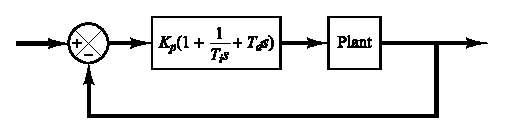
\includegraphics[width=8cm]{images/PIDController.eps}
\begin{itemize}
	\item Controlador PID $\rightarrow$ Depende de los parámetros $K_p$, $T_i$, $T_d$.
	\item \textbf{Sintonización:} Selección de valores numéricos para los parámetros, con base en algún criterio.
	\item Existen muchos criterios para sintonización de controladores.
	\begin{itemize}
		\item Experimentales
		\item Análisis de la función de transferencia
		\item Técnicas de optimización
		\item Lugar geométrico de las raíces
		\item Compensación en frecuencia
	\end{itemize}
\end{itemize}
\end{frame}

\section{Criterios Clásicos de Sintonización}
\subsection{Método de Ziegler-Nichols}
\begin{frame}[<+->]\frametitle{Método de Ziegler-Nichols}
\begin{itemize}
	\item Método experimental.
	\item Útil cuando no se conoce un modelo matemático detallado de la planta.
	\item Está diseñado para proveer un buen rechazo a perturbaciones.
	\item Produce un sobrepico grande.
	\item Los parámetros resultantes no necesariamente son óptimos. Se toman como punto de partida para un ajuste fino.
	\item Dos métodos
	\begin{enumerate}
		\item Lazo abierto: Características de la curva de reacción ante entrada paso.
		\item Lazo cerrado: Aumentar la ganancia proporcional hasta un valor crítico.
	\end{enumerate}
\end{itemize}
\end{frame}

\begin{frame}[<+->]\frametitle{Método de Ziegler-Nichols / Método 1: Lazo Abierto}
\small
\vspace*{-2mm}
\begin{columns}
\begin{column}{0.5\textwidth}
\begin{itemize}
	\item Aplicar entrada paso unitaria al sistema y medir la respuesta (experimental o simulación).
	\item Si la respuesta tiene forma de $S$, se puede aplicar el método.
	\item Caracterizar la curva obtenida usando dos parámetros: tiempo muerto $L$ y constante de tiempo $T$.
	\item Los parámetros se encuentran dibujando una recta tangente al punto de inflexión de la curva en forma de $S$.
\end{itemize}
\end{column}	
\begin{column}{0.5\textwidth}
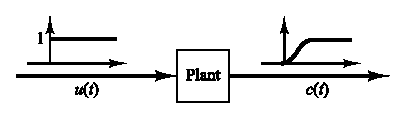
\includegraphics[width=6.5cm]{images/zieglerNichols1a.eps}\\
\vspace*{5mm}
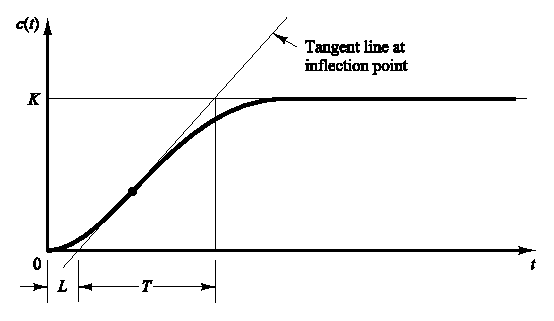
\includegraphics[width=6.5cm]{images/zieglerNichols1b.eps}
\end{column}	
\end{columns}
\end{frame}

\begin{frame}[<+->]\frametitle{Método de Ziegler-Nichols / Método 1: Lazo Abierto}
\begin{columns}
\begin{column}{0.5\textwidth}
\small
\begin{itemize}
	\item La función de transferencia $C(s)/U(s)$ se puede aproximar a un sistema de primer orden mas tiempo muerto:
	\begin{equation*}
		\frac{C(s)}{U(s)} = \frac{K e^{-Ls}}{Ts + 1}
	\end{equation*}
	\item Ziegler y Nichols sugirieron asignar los valores para los parámetros de acuerdo con la siguiente tabla:
	\begin{table}
	\begin{tabular}{c|c|c|c}
		Controlador & $K_p$ & $T_i$ & $T_d$\\
		\hline
		P   & $T/L$ & $\infty$ & 0\\
		PI  & $0.9T/L$ & $L/0.3$ & 0\\
		PID & $1.2T/L$ & $2L$ & $0.5L$
	\end{tabular}
	\end{table}
\end{itemize}
\end{column}	
\begin{column}{0.5\textwidth}
Note que el controlador PID obtenido por éste método tiene la forma:
\begin{align*}
	G_c(s) &= K_p\left( 1 + \frac{1}{T_i s} + T_d s \right)\\
	&= 1.2\frac{T}{L}\left( 1 + \frac{1}{2Ls} + 0.5 Ls \right)\\
	&= 0.6T \frac{\left( s + \frac{1}{L} \right)^2}{s}
\end{align*}
El controlador PID tiene un polo en el origen y doble cero en $s = -1/L$.
\end{column}	
\end{columns}
\end{frame}

\begin{frame}[<+->]\frametitle{Método de Ziegler-Nichols / Método 2: Lazo Cerrado}
\begin{columns}
\begin{column}{0.5\textwidth}
	\begin{itemize}
		\item Se inicia configurando $T_i = \infty$ y $T_d = 0$.
		\item Usando sólo acción proporcional, aumentar $K_p$ desde 0 hasta un valor crítico $K_{cr}$ en el cual la salida presenta oscilaciones sostenidas.
		\item Si no se obtienen oscilaciones, el método no se puede aplicar.
		\item A partir del experimento se determinan la ganancia crítica $K_{cr}$ y periodo crítico $P_{cr}$.
	\end{itemize}	
\end{column}	
\begin{column}{0.5\textwidth}
	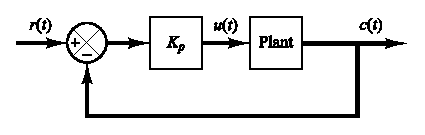
\includegraphics[width=6.5cm]{images/zieglerNichols2a.eps}\\
	\vspace*{5mm}
	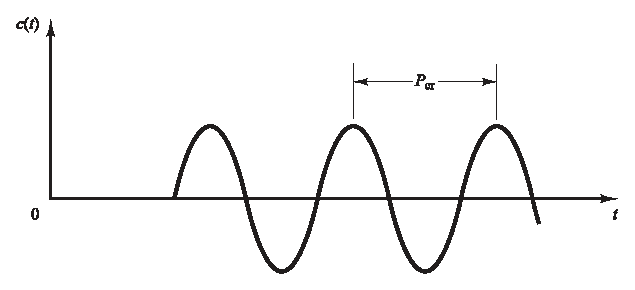
\includegraphics[width=6.5cm]{images/zieglerNichols2b.eps}
\end{column}	
\end{columns}
\end{frame}
\small
\begin{frame}[<+->]\frametitle{Método de Ziegler-Nichols / Método 2: Lazo Cerrado}
\begin{columns}
\begin{column}{0.5\textwidth}
	Ziegler y Nichols sugirieron asignar los valores para los parámetros de acuerdo con la siguiente tabla:
	\footnotesize
	\begin{table}
	\begin{tabular}{c|c|c|c}
		Controlador & $K_p$ & $T_i$ & $T_d$\\
		\hline
		P   & $0.5  K_{cr}$ & $\infty$ & 0\\
		PI  & $0.45 K_{cr}$ & $P_{cr}/1.2$ & 0\\
		PID & $0.6  K_{cr}$ & $P_{cr}/2$ & $0.125P_{cr}$
	\end{tabular}
	\end{table}
\end{column}	
\begin{column}{0.5\textwidth}
\small
Note que el controlador PID obtenido por el segundo método tiene la forma:
\begin{align*}
	G_c(s) &= K_p\left( 1 + \frac{1}{T_i s} + T_d s \right)\\
	&= 0.6 K_{cr} \left( 1 + \frac{1}{0.5 P_{cr}s} + 0.125 P_{cr}s \right)\\
	&= 0.075K_{cr}P_{cr} \frac{\left( s + \frac{4}{P_{cr}} \right)^2}{s}
\end{align*}
Entonces, el controlador PID tiene un polo en el origen y doble cero en $s = -4/P_{cr}$.
\end{column}	
\end{columns}
\end{frame}

\begin{frame}[<+->]\frametitle{Método de Ziegler-Nichols / Ejemplo}
Considere el sistema de control mostrado en la figura. Usando el método de Ziegler-Nichols, determine los parámetros del controlador PID tal que se obtenga un sobrepico máximo de aproximadamente 25\%. Si el sobrepico máximo es excesivo, realice un ajuste fino para reducirlo.
\begin{figure}
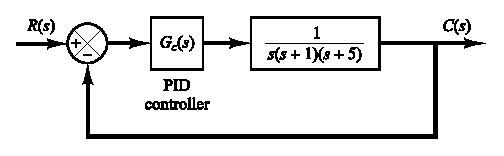
\includegraphics[width=8cm]{images/ejemplo1.eps}
\end{figure}
\end{frame}

\begin{frame}[<+->]\frametitle{Método de Ziegler-Nichols / Ejemplo}
\begin{itemize}
	\item Dado que la planta tiene un integrador, se utiliza el segundo método.
	\item Definiendo $T_i = \infty$ y $T_d = 0$, se obtiene la función de transferencia de lazo cerrado:
	\begin{equation*}
		\frac{C(s)}{R(s)} = \frac{K_p}{s(s+1)(s+5) + K_p} = \frac{K_p}{s^3 + 6s^2 + 5s + K_p}
	\end{equation*}
	\item El valor crítico de $K_p$ para obtener oscilaciones sostenidas se puede obtener usando el criterio de estabilidad de Routh-Hurwitz para el polinomio característico $q(s) = s^3 + 6s^2 + 5s + K_p = 0$:
	\begin{columns}
	\begin{column}{0.4\textwidth}
		\begin{table}
		\begin{tabular}{c|cc}
			$s^3$ & 1 & 5\\
			$s^2$ & 6 & $K_p$\\
			$s^1$ & $\frac{30-K_p}{6}$ & \\
			$s^0$ & $K_p$ & 
		\end{tabular}
		\end{table}
	\end{column}	
	\begin{column}{0.6\textwidth}
		\begin{itemize}
			\item El valor crítico de $K_p$ para obtener oscilaciones sostenidas es $K_{cr} = 30$.
			\item En éste caso, el polinomio característico es $q(s) = s^3 + 6s^2 + 5s + 30 = 0$.
		\end{itemize}
	\end{column}	
	\end{columns}
\end{itemize}
\end{frame}

\begin{frame}[<+->]\frametitle{Método de Ziegler-Nichols / Ejemplo}
\begin{columns}
\begin{column}{0.5\textwidth}
\small
\begin{itemize}
	\item Para hallar la frecuencia de la oscilación se substituye $s = j\omega$ en el polinomio característico:
	\begin{align*}
		(j\omega)^3 + 6(j\omega)^2 + 5(j\omega) + 30 = 0\\
		6(5 - \omega^2) + j\omega(5-\omega^2) = 0\\
		\Rightarrow \omega = \sqrt{5}
	\end{align*}
	\item El periodo de oscilación sostenida es:
	\begin{equation*}
		P_{cr} = \frac{2\pi}{\omega} = \frac{2\pi}{\sqrt{5}} = 2.8099
	\end{equation*}
\end{itemize}
\end{column}
\begin{column}{0.5\textwidth}
\small
\begin{itemize}
	\item Usando la tabla para el método 2, se obtienen los valores del controlador PID como:
	\begin{align*}
		K_p &= 0.6 K_{cr} = 18\\
		T_i &= 0.5 P_{cr} = 1.405\\
		T_d &= 0.125P_{cr} = 0.35124
	\end{align*}
	\item La función de transferencia del controlador PID queda:
	\begin{align*}
		G_c(s) &= 18 \left( 1 + \frac{1}{1.405s} + 0.35124 s \right)\\
		&= \frac{6.3223(s+1.4235)^2}{s}
	\end{align*}
\end{itemize}
\end{column}
\end{columns}
\end{frame}

\begin{frame}[<+->]\frametitle{Método de Ziegler-Nichols / Ejemplo}
\vspace*{5mm}
\begin{columns}
\begin{column}{0.5\textwidth}
	La respuesta del sistema en lazo cerrado ante una entrada paso es:
	\begin{figure}
		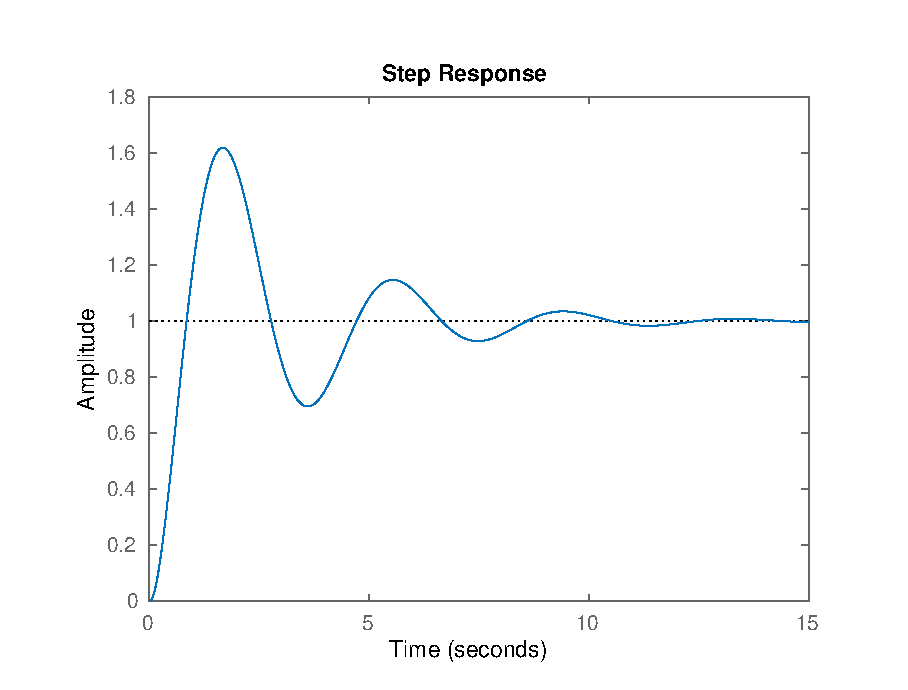
\includegraphics[width=7cm]{images/ejemplo1Respuesta.eps}
	\end{figure}
\end{column}	
\begin{column}{0.5\textwidth}
	Sobrepico 60\% approximadamente $\rightarrow$ se require ajustar los parámetros para disminuir el sobrepico:
	\begin{align*}
		K_p = 39.42\\
		T_i = 3.077\\
		T_d = 0.7692
	\end{align*}
\end{column}	
\end{columns}
\end{frame}

\subsection{Método de Cohen-Coon}
\begin{frame}[<+->]\frametitle{Método de Cohen-Coon}
  \begin{itemize}
 		\item Ziegler-Nichols: sensible a la relación $L/T$.
   	\item Cohen-Coon: Mejora el desempeño cuando el tiempo muerto es comparable a la constante de tiempo.
  \end{itemize}
  \begin{table}
  	\begin{tabular}{c|c|c|c}
  		Controlador & $K_p$ & $T_i$ & $T_d$\\
  		\hline
  		P   & $\frac{T}{K_0 L}\left(1   + \frac{L}{3T} \right)$ & $\infty$ & 0\\
  		PI  & $\frac{T}{K_0 L}\left(0.9 + \frac{L}{12T} \right)$ & $L \frac{30T+3L}{9T+20L}$ & 0\\
  		PID & $\frac{T}{K_0 L}\left(\frac{4}{3} + \frac{L}{4T} \right)$ & $L \frac{32T+6L}{13T+8L}$ & $\frac{4TL}{11T+22}$
  	\end{tabular}
  \end{table}
  \begin{equation*}
  	K_0 = \frac{\Delta c}{\Delta u}
  \end{equation*}
\end{frame}

\section{Sintonía Óptima de Controladores}
\subsection{Índices de Desempeño}
\begin{frame}[<+->]\frametitle{Índices de Desempeño}
	Sistema de control óptimo: los parámetros del sistema se ajustan para minimizar (maximizar) un índice de desempeño.
	\begin{columns}
	\begin{column}{0.5\textwidth}
	\begin{itemize}
		\item Integral del cuadrado del error (ISE):
		\begin{equation*}
			ISE = \int_0^T e^2(t) dt
		\end{equation*}
		\item Integral del valor absoluto del error (IAE):
		\begin{equation*}
			IAE = \int_0^T |e(t)| dt
		\end{equation*}
	\end{itemize}
	\end{column}	
	\begin{column}{0.5\textwidth}
	\begin{itemize}
		\item Integral del valor absoluto del error ponderado en el tiempo (ITAE):
		\begin{equation*}
			ITAE = \int_0^T t |e(t)| dt
		\end{equation*}
		\item Integral del cuadrado del error ponderado en el tiempo (ITSE):
		\begin{equation*}
			ITAE = \int_0^T t e^2(t) dt
		\end{equation*}
	\end{itemize}
	\end{column}	
	\end{columns}
	\vspace*{-5mm}
	$T$: Es conveniente seleccionarlo como el tiempo de establecimiento $T_s$.
\end{frame}

\begin{frame}[<+->]\frametitle{Índices de Desempeño}
	\begin{itemize}
		\item ISE: otorga más peso a errores grandes, lo cual usualmente ocurre al inicio de la respuesta, y menos peso a errores pequeños, lo cual ocurre normalmente hacia el final de la respuesta.
		\item ISE: produce ganancias del controlador grandes y respuestas muy oscilatorias.
		\item ITAE, ITSE: agrega un término de penalización asociado al tiempo transcurrido.
		\item Lopez et al [1967] desarrollaron fórmulas empíricas de mínimo error integral.
		\item Aplicables para el intervalo $0.1 < L/T < 1$.
	\end{itemize}
\end{frame}

\begin{frame}[<+->]\frametitle{Sintonización Óptima para Regulación - Controlador P}
\begin{figure}
	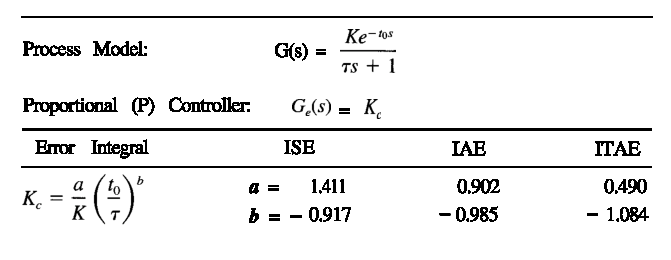
\includegraphics[width=9cm]{images/criteriosOptimosP.eps}
\end{figure}
\end{frame}

\begin{frame}[<+->]\frametitle{Sintonización Óptima para Regulación - Controlador PI}
\begin{figure}
	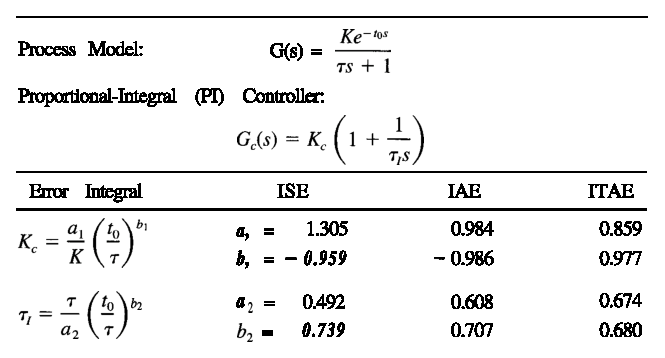
\includegraphics[width=9cm]{images/criteriosOptimosPI.eps}
\end{figure}
\end{frame}

\begin{frame}[<+->]\frametitle{Sintonización Óptima para Regulación - Controlador PID}
\begin{figure}
	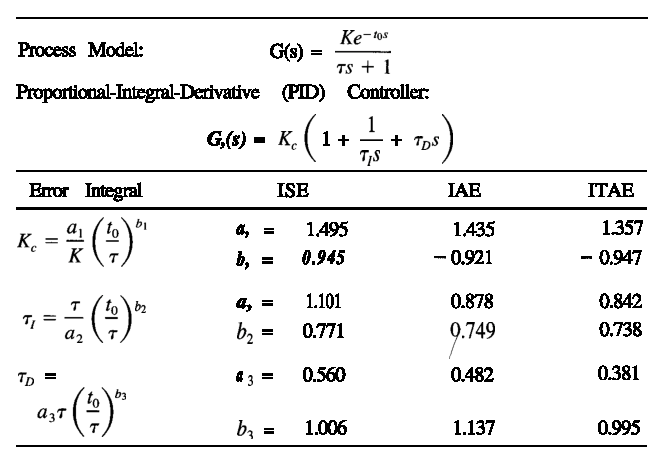
\includegraphics[width=9cm]{images/criteriosOptimosPID.eps}
\end{figure}
\end{frame}

\begin{frame}[<+->]\frametitle{Sintonización Óptima para Servos - Controlador PI}
\begin{figure}
	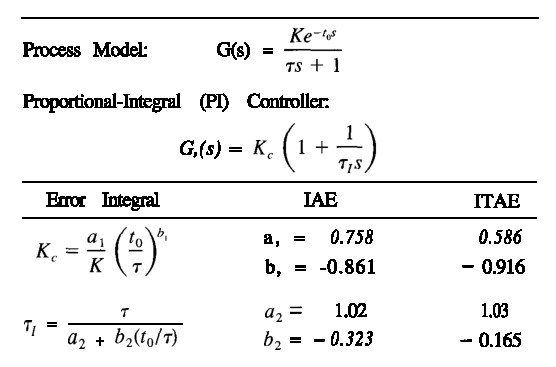
\includegraphics[width=9cm]{images/criteriosOptimosServoPI.eps}
\end{figure}
\end{frame}

\begin{frame}[<+->]\frametitle{Sintonización Óptima para Servos - Controlador PID}
\begin{figure}
	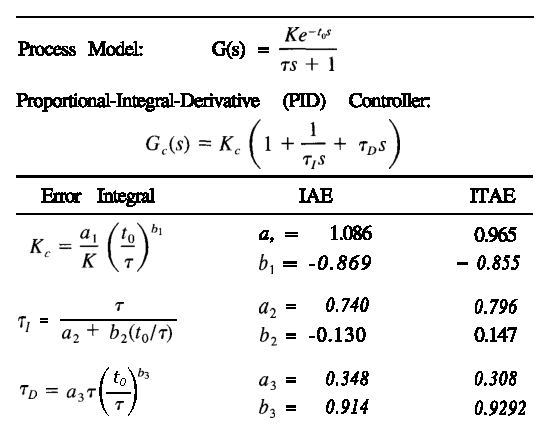
\includegraphics[width=8cm]{images/criteriosOptimosServoPID.eps}
\end{figure}
\end{frame}

\begin{frame}[c]\frametitle{Taller}
	\begin{enumerate}
		\item Considere el sistema de control mostrado en la figura.
		\begin{itemize}
			\item Diseñe un controlador PID usando el método de Ziegler-Nichols.
			\item Determine la respuesta a entrada unitaria y disturbio unitario.
			\item Cuál es el máximo sobrepico y tiempo de establecimiento para la respuesta a entrada unitaria?
		\end{itemize}
		\seti
	\end{enumerate}
	\begin{figure}
		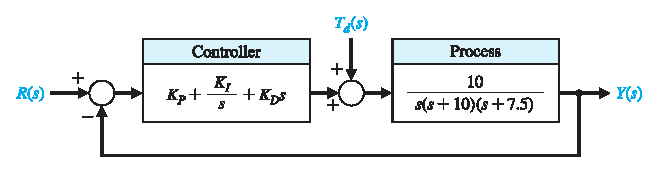
\includegraphics[width=10cm]{images/ejercicio1.eps}
	\end{figure}
\end{frame}

\begin{frame}[c]\frametitle{Taller}
	\begin{enumerate}
		\conti
		\item La siguiente figura muestra la curva de reacción obtenida al aplicar una entrada paso al sistema $G(s) = \frac{1}{(s+1)^4}$.
		\vspace*{-5mm}
		\begin{columns}
		\begin{column}{0.5\textwidth}
		\begin{figure}
			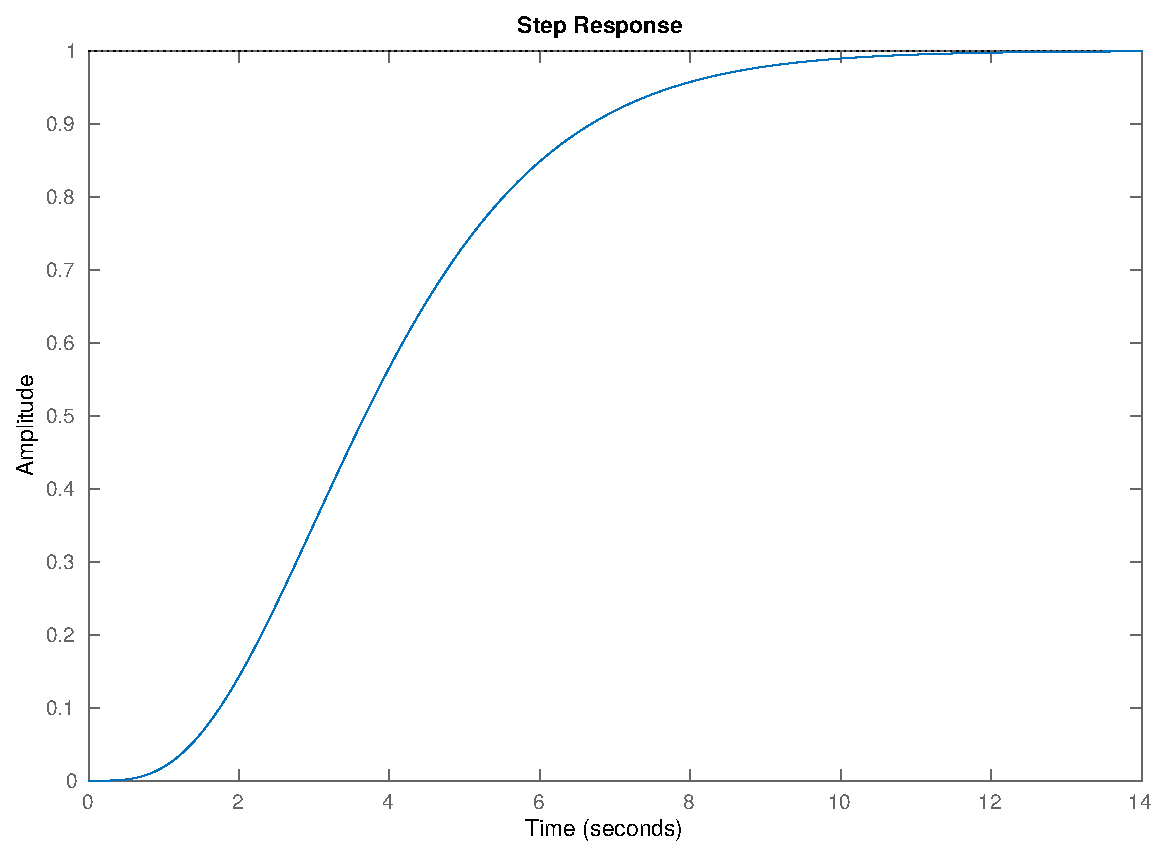
\includegraphics[width=7cm]{images/responseCurve.eps}
		\end{figure}
		\end{column}	
		\begin{column}{0.5\textwidth}
		\begin{itemize}
			\item Encuentre una aproximación de primer orden mas tiempo muerto (FOPDT) para el sistema.
			\item Diseñe un controlador PID usando los métodos de Ziegler-Nichols, Cohen-Coon e ITAE.
			\item Compare los valores de los parámetros obtenidos en cada caso.
			\item Evalue el desempeño de cada controlador ante entrada paso unitario y disturbio paso unitario.
		\end{itemize}
		\end{column}	
		\end{columns}
		\seti
	\end{enumerate}
\end{frame}

% \begin{frame}[<+->]\frametitle{Controlador ON-OFF / BANG-BANG / TODO-NADA}
% \begin{columns}
%   \begin{column}{0.5\textwidth}
%     \vspace*{5mm}
%     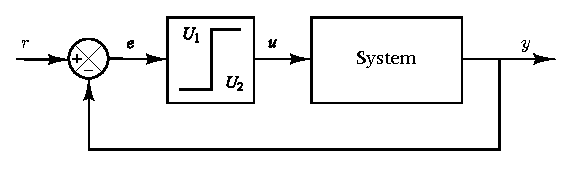
\includegraphics[width=7cm]{images/onoffcontroller.eps}
%     \vspace*{-5mm}
%     \begin{itemize}
%       \item Se caracteriza porque el actuador posee sólo dos posiciones: encendido - apagado.
%       \item Ventajas:
%       \begin{itemize}
%         \item Implementación simple.
%         \item Implementación barata.
%         \item Uso común en aplicaciones domésticas.
%       \end{itemize}
%     \end{itemize}
%   \end{column} 
%   \begin{column}{0.5\textwidth}
%     \begin{align*}
%       u(t) =
%       \begin{cases}
%         U_1 & \text{si } e(t) > 0\\
%         U_2 & \text{si } e(t) < 0\\
%       \end{cases}
%     \end{align*}
%     \begin{itemize}
%       \item En la práctica generalmente no se usa éste controlador $\rightarrow$ puede provocar muchas conmutaciones $\rightarrow$ puede producir desgaste en el actuador.
%       \item En su lugar se usa un controlador con histéresis.
%     \end{itemize}
%   \end{column} 
% \end{columns}
% \end{frame}

% \begin{frame}[<+->]\frametitle{Controlador ON-OFF con Histéresis}
% \begin{columns}
%   \begin{column}{0.5\textwidth}
%     \vspace*{5mm}
%     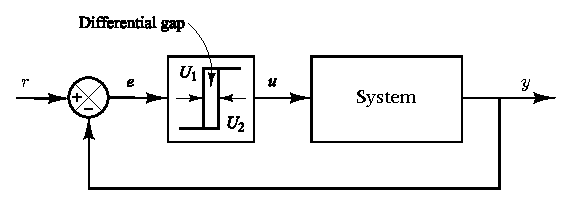
\includegraphics[width=7cm]{images/onoffcontrollerHisteresis.eps}
%     \vspace*{-5mm}
%     \begin{itemize}
%       \item Permite mantener el valor presente de $u(t)$ hasta que la señal de error se haya movido más allá del valor cero.
%       \item La amplitud de la oscilación puede reducirse disminuyendo la brecha diferencial $\rightarrow$ más conmutaciones.
%     \end{itemize}
%   \end{column} 
%   \begin{column}{0.5\textwidth}
%     \begin{center}
%     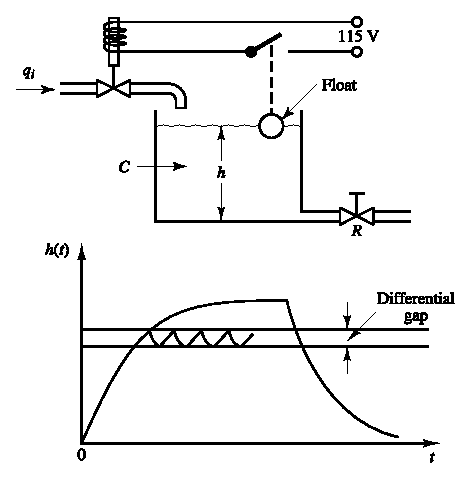
\includegraphics[width=5.5cm]{images/onoffcontrollerLevel.eps}
%     \end{center}
%     \vspace*{-5mm}
%     \begin{itemize}
%       \item No se puede utilizar para modificar transitorios.
%     \end{itemize}
%   \end{column} 
% \end{columns}
% \end{frame}

% \begin{frame}[<+->]\frametitle{Controlador Proporcional (P)}
% \begin{columns}
%   \begin{column}{0.5\textwidth}
%     \vspace*{5mm}
%     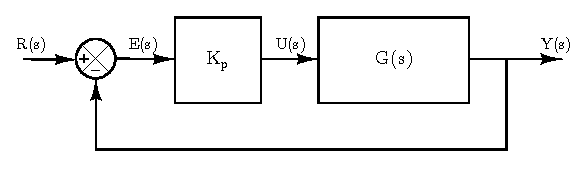
\includegraphics[width=7cm]{images/Pcontroller.eps}
%     \vspace*{-5mm}
%     \begin{itemize}
%       \item Es un amplificador de error.
%       \begin{align*}
%         U(s) = K_p E(s)
%       \end{align*}
%       \item Dependencia de $E(s)$ de la ganancia $K_p$:
%       \begin{align*}
%         E(s) = \frac{1}{1+K_p G(s)}R(s)
%       \end{align*}
%     \end{itemize}
%   \end{column} 
%   \begin{column}{0.5\textwidth}
%     \begin{itemize}
%       \item $K_p$ aumenta $\Rightarrow$ menor error de estado estacionario.
%       \item $K_p$ muy grande no elimina el error de estado estacionario:
%       \item $K_p$ muy grande puede ocasionar inestabilidad.
%     \end{itemize}
%   \end{column} 
% \end{columns}
% \end{frame}

% \begin{frame}[<+->]\frametitle{Controlador Proporcional (P) - Error de Estado Estacionario}
%   \begin{align*}
%     E(s) = \frac{1}{1+K_p G(s)}R(s)
%   \end{align*}
%   \pause
%   Asumiendo $G(s)$ de la forma:
%   \begin{align*}
%     G(s) = \frac{a_n s^n + a_{n-1} s^{n-1} + \dots + a_1 s + a_0}{b_m s^m + b_{m-1} s^{m-1} + \dots + b_1 s + b_0}
%   \end{align*}
%   \pause
%   Usando el teorema del valor final: 
%   \begin{align*}
%     e_{ss} = \lim_{s \rightarrow 0} s \left(\frac{1}{s}\right) \left(\frac{1}{1 + K_p G(s)}\right) = \frac{1}{1 + K_p \frac{a_0}{b_0}}
%   \end{align*}
% \end{frame}

% \begin{frame}[<+->]\frametitle{Controlador Proporcional (P) - Ejemplo}
%   Suponga  $G(s) = \frac{1}{s+a}$. Entonces la ganancia de lazo cerrado será:
%   \begin{align*}
%     G_{lc}(s) = \frac{K_p}{s+a+K_p}
%   \end{align*}
%   \pause
%   Si $R(s) = 1/s$ (escalón unitario) entonces:
%   \begin{align*}
%     Y(s) = \left(\frac{K_p}{s+a+K_p}\right) \frac{1}{s}
%   \end{align*}
%   \pause
%   Aplicando la transformada inversa de Laplace:
%   \begin{equation*}
%     y(t) = \frac{K_p}{K_p+a} \left(1-e^{-t(K_p+a)}\right)
%   \end{equation*}
%   \pause
%   Si $K_p$ se incrementa, el sistema será más rápido (no es el caso general).
% \end{frame}

% \begin{frame}[<+->]\frametitle{Controlador Proporcional (P) - Rechazo a Perturbaciones}
% \begin{columns}
% \begin{column}{0.5\textwidth}
% \vspace*{-3mm}
% \begin{center}
%   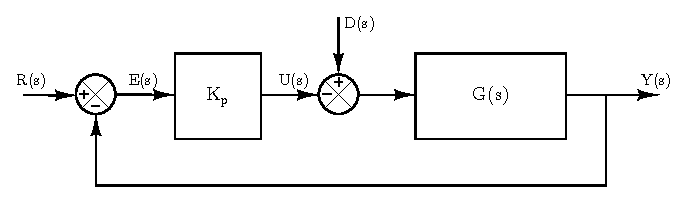
\includegraphics[width=7.5cm]{images/PcontrollerwithDisturbance.eps}\\
% \end{center}
% \pause
% Asumiendo $R(s) = 0$:
% \begin{equation*}
%   \frac{Y(s)}{D(s)} = \frac{G(s)}{1 + K_p G(s)}
% \end{equation*}
% \pause
% Asumiendo $G(s)$ de la forma:
% \begin{align*}
%   G(s) = \frac{a_n s^n + a_{n-1} s^{n-1} + \dots + a_1 s + a_0}{b_m s^m + b_{m-1} s^{m-1} + \dots + b_1 s + b_0}
% \end{align*}
% \end{column}
% \pause
% \begin{column}{0.5\textwidth}
%   Usando el teorema del valor final, asumiendo perturbación constante: 
%   \begin{align*}
%     y_{ss} &= \lim_{s \rightarrow 0} s \left(\frac{1}{s}\right) \left(\frac{G(s)}{1 + K_p G(s)}\right)\\
%     &= \frac{a_0}{b_0 + K_p a_0}
%   \end{align*}
%   \pause
%   Incrementar $K_p$ reduce el efecto de la perturbación, pero no lo elimina. No es inmune al ruido.
% \end{column}
% \end{columns}
% \end{frame}

% \begin{frame}[<+->]\frametitle{Controlador Proporcional (P) - Ventajas y Desventajas}
%   \begin{itemize}
%     \item Ventajas:
%     \begin{itemize}
%       \item Instantaneidad de aplicación.
%       \item Facilidad para comprobar resultados.
%     \end{itemize}
%     \item Desventajas:
%     \begin{itemize}
%       \item Falta de inmunidad a ruido.
%       \item No corrige algunos errores en estado estacionario.
%       \item Puede hacer inestable al sistema.
%     \end{itemize}
%   \end{itemize}
% \end{frame}

% \begin{frame}[<+->]\frametitle{Controlador Integral (I)}
% % \vspace*{-5mm}
% \begin{columns}
% \begin{column}{0.5\textwidth}
% \begin{center}
%   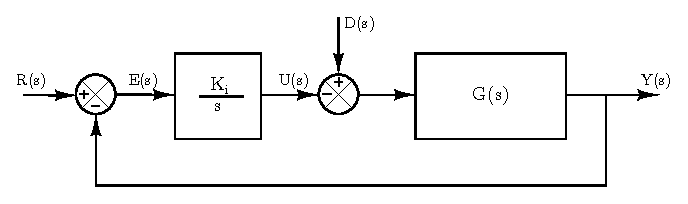
\includegraphics[width=7cm]{images/Icontroller.eps}
% \end{center}
% \pause
% \begin{equation*}
%   u(t) = \int_0^t e(t) dt \longrightarrow \frac{U(s)}{E(s)} = \frac{K_i}{s}
% \end{equation*}
% \pause
% Ganancia de lazo cerrado:
% \begin{equation*}
%   G_{lc}(s) = \frac{Y(s)}{R(s)} = \frac{K_i G(s)}{s + K_i G(s)}
% \end{equation*}
% \pause
% Dependencia de $E(s)$ de la ganancia $K_i$:
% \begin{equation*}
% E(s) = (1-G_{lc}(s)) = \frac{s}{s+K_i G(s)} R(s)
% \end{equation*}
% \pause
% \end{column}
% \begin{column}{0.5\textwidth}
% Asumiendo $G(s)$ de la forma:
% \begin{align*}
%   G(s) = \frac{a_n s^n + a_{n-1} s^{n-1} + \dots + a_1 s + a_0}{b_m s^m + b_{m-1} s^{m-1} + \dots + b_1 s + b_0}
% \end{align*}
% \pause
% Usando el teorema del valor final:
% \begin{equation*}
%   e_{ss} = \lim_{s \rightarrow 0} s \frac{s}{s + K_i \frac{a_n s^n + a_{n-1} s^{n-1} + \dots + a_1 s + a_0}{b_m s^m + b_{m-1} s^{m-1} + \dots + b_1 s + b_0}}R(s) 
% \end{equation*}
% \pause
% Si $R(s) = 1/s$, entonces $e_{ss} = 0$.\\
% \textbf{El integrador anula el error de estado estable.}
% \end{column}
% \end{columns}
% \end{frame}

% \begin{frame}[<+->]\frametitle{Controlador Integral (I) - Rechazo a Perturbaciones}
% \begin{align*}
%   \frac{Y(s)}{D(s)} &= \frac{G(s)}{1+\frac{K_i}{s}G(s)} = \frac{\frac{a_n s^n + \dots + a_0}{b_m s^m + \dots + b_0}}{1 + \frac{K_i}{s}\frac{a_n s^n + \dots + a_0}{b_m s^m + \dots + b_0}}\\
%   &= \frac{(a_n s^n + \dots + a_0)s}{(b_m s^m + \dots + b_0)s + K_i(a_n s^n + \dots + a_0)} 
% \end{align*}
% \pause
% Si $D(s) = 1/s$ (escalón unitario), entonces
% \begin{equation*}
%   y_{ss} = \lim_{s \rightarrow 0} s \frac{1}{s} \frac{(a_n s^n + \dots + a_0)s}{(b_m s^m + \dots + b_0)s + K_i(a_n s^n + \dots + a_0)} = 0
% \end{equation*}
% \pause
% \textbf{El integrador elimina perturbaciones en estado estacionario.}
% \end{frame}

% \begin{frame}[<+->]\frametitle{Controlador Integral (I) - Ventajas y Desventajas}
%   \begin{itemize}
%     \item Ventajas:
%     \begin{itemize}
%       \item Elimina error de estado estacionario.
%       \item Elimina efecto de las perturbaciones (robustez).
%     \end{itemize}
%     \item Desventajas:
%     \begin{itemize}
%       \item La aplicación no es instantánea.
%       \item Puede agregar inestabilidad al sistema total debido al polo en el origen.
%     \end{itemize}
%   \end{itemize}
% \end{frame}

% \begin{frame}[<+->]\frametitle{Controlador Proporcional - Integral (PI)}
% \begin{center}
%   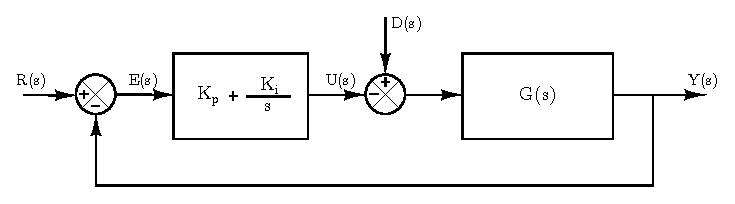
\includegraphics[width=8cm]{images/PIcontroller.eps}
% \end{center}
% \pause
% \begin{equation*}
%   u(t) = K_p e(t) + K_i \int_0^t e(t) dt \longrightarrow U(s) = K_p E(s) + K_i \frac{E(s)}{s}
% \end{equation*}
% \pause
% \begin{equation*}
%   \frac{U(s)}{E(s)} = K_p + \frac{K_i}{s} = \frac{K_p s + K_i}{s}
% \end{equation*}
% % \pause
% % \begin{equation*}
% %   \frac{U(s)}{E(s)} = K_p \left(1 + \frac{1}{T_i s} \right),\ T_i\text{: Tiempo integral}
% % \end{equation*}
% \end{frame}

% \begin{frame}[<+->]\frametitle{Controlador Proporcional - Integral (PI)}
% \begin{align*}
%   G_{lc}(s) = \frac{Y(s)}{R(s)} = \frac{\frac{K_ps + K_i}{s}G(s)}{1 + \frac{K_ps + K_i}{s}G(s)} = \frac{(K_ps + K_i)G(s)}{s + (K_ps+K_i)G(s)}
% \end{align*}
% \pause
% \begin{align*}
%   E(s) = R(s) - Y(s) = R(s) - G_{lc}(s)R(s)
% \end{align*}
% \pause
% \begin{align*}
%   \frac{E(s)}{R(s)} = 1 - G_{lc}(s) = 1 - \frac{(K_ps + K_i)G(s)}{s + (K_ps+K_i)G(s)} = \frac{s}{s + (K_ps + K_i)G(s)}
% \end{align*}
% \pause
% Aplicando el teorema del valor final:
% \begin{equation*}
%   e_{ss} = \lim_{s \rightarrow 0} s \frac{s}{s + (K_ps + K_i)G(s)} R(s)
% \end{equation*}
% \pause
% Si $R(s) = 1/s$ (escalón unitario), entonces $e_{ss} = 0$. \textbf{El controlador anula el error de estado estacionario.}
% \end{frame}

% \begin{frame}[<+->]\frametitle{Controlador Proporcional - Integral (PI) - Rechazo a Perturbaciones}
% \begin{equation*}
%   \frac{Y(s)}{D(s)} = \frac{G(s)}{1 + G(s)\frac{K_ps + K_i}{s}} = \frac{G(s)s}{s + G(s)(K_ps+K_i)}
% \end{equation*}
% \pause
% Si $D(s) = 1/s$, entonces:
% \begin{equation*}
%   y_{ss} = \lim_{s \rightarrow 0} s \frac{1}{s} \frac{G(s)s}{s + G(s)(K_ps+K_i)} = 0
% \end{equation*}
% \pause
% \textbf{El controlador elimina el efecto de las perturbaciones.}
% \end{frame}

% \begin{frame}[<+->]\frametitle{Controlador Proporcional - Integral (PI) - Ventajas}
% \begin{itemize}
%   \item Respuesta inmediata
%   \item Elimina error de estado estacionario.
%   \item Elimina efecto de las perturbaciones (robustez).
% \end{itemize}
% \end{frame}

% \begin{frame}[<+->]\frametitle{Control Derivativo (D)}
% \begin{center}
%   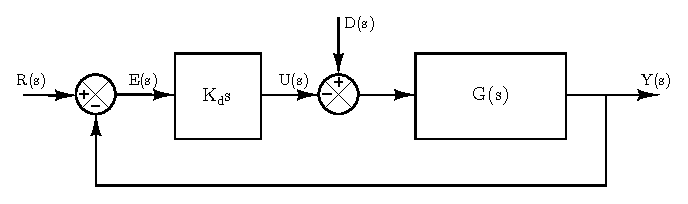
\includegraphics[width=8cm]{images/Dcontroller.eps}
% \end{center}
% \pause
% \begin{equation*}
%   u(t) = K_d \frac{de(t)}{dt} \longrightarrow U(s) = K_d s E(s) \rightarrow \frac{U(s)}{E(s)} = K_d s
% \end{equation*}
% \pause
% \begin{align*}
%   \frac{E(s)}{R(s)} = 1 - G_{lc}(s) = 1 - \frac{G(s) K_d s}{1 + G(s) K_d s} = \frac{1}{1 + K_d s G(s)}
% \end{align*}
% \pause
% \begin{equation*}
%   e_{ss} = \lim_{s \rightarrow 0} s \frac{A}{s} \frac{1}{1 + K_d s G(s)} = A
% \end{equation*}
% \pause
% \textbf{No elimina el error de estado estacionario!}
% \end{frame}

% \begin{frame}[<+->]\frametitle{Control Derivativo (D) - Rechazo a Perturbaciones}
% Si $R(s) = 0$:
% \begin{equation*}
%   \frac{Y(s)}{D(s)} = \frac{G(s)}{1 + G(s) K_d s}
% \end{equation*}
% \pause
% Asumiendo $D(s) = A/s$:
% \begin{equation*}
%   y_{ss} = \lim_{s \rightarrow 0} s \frac{A_p}{s} \frac{G(s)}{1 + G(s) K_d s} = A_p G(s)
% \end{equation*}
% \pause
% \textbf{No elimina perturbaciones!}
% \end{frame}

% \begin{frame}[<+->]\frametitle{Control Derivativo (D) - Análisis en Tiempo}
% \begin{columns}
% \begin{column}{0.3\textwidth}
% \begin{center}
%   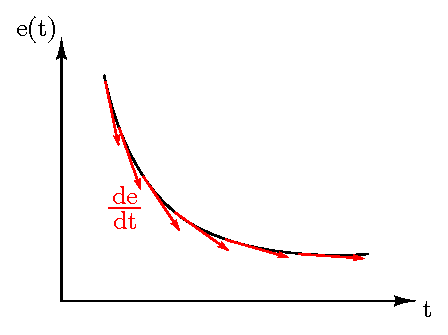
\includegraphics[width=5cm]{images/Dcontroller_time.eps}
% \end{center}
% \end{column} 
% \begin{column}{0.7\textwidth}
%   \begin{itemize}
%     \item Debido a la dinámica del proceso, pasa algún tiempo hasta que cambios en la variable de control produzcan cambios en la salida del proceso.
%     \item La acción derivativa trata de \textit{predecir} o \textit{anticipar} el valor que tomará la señal de error para dar un valor a la señal de control.
%     \item Ventaja: Es anticipativo. adelanta la acción de control frente a la aparición de una tendencia del error (sólo aplica a transitorios).
%     \item Desventaja: Inaplicable ante la presencia de ruido.
%   \end{itemize}
% \end{column} 
% \end{columns}
% \end{frame}

% \begin{frame}[<+->]\frametitle{Control Proporcional - Derivativo (PD)}
% \begin{center}
%   \includegraphics[width=8cm]{images/PDcontroller.eps}
% \end{center}
% \pause
% \begin{equation*}
%   u(t) = K_p e(t) + K_d \frac{de(t)}{dt} \longrightarrow U(s) = K_p E(s) + K_d s E(s) \rightarrow \frac{U(s)}{E(s)} = K_p + K_d s
% \end{equation*}
% \begin{columns}
% \begin{column}{0.5\textwidth}
% Ventajas:
% \begin{itemize}
%   \item Reduce el error de estado estable.
%   \item Adelanta la acción de control (es anticipativo).
%   \item La respuesta es inmediata.
% \end{itemize}
% \end{column}
% \begin{column}{0.5\textwidth}
% Desventajas:
% \begin{itemize}
%   \item No corrije errores en estado estacionario.
%   \item Es sensible a ruidos. Generalmente se utiliza con un filtro en la entrada.
% \end{itemize}
% \end{column}
% \end{columns}
% \end{frame}

% \begin{frame}[<+->]\frametitle{Control Proporcional - Integral - Derivativo (PID)}
% \begin{center}
%   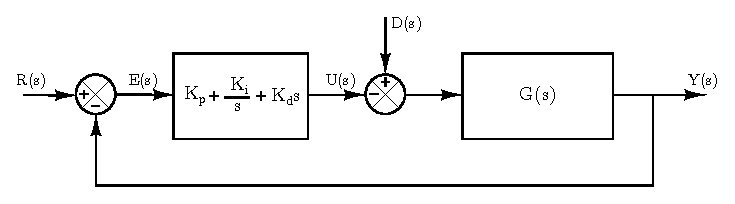
\includegraphics[width=8cm]{images/PIDcontroller.eps}
% \end{center}
% \pause
% \begin{align*}
%   u(t) = K_p e(t) + K_i \int_0^t e(t) dt + K_d \frac{de(t)}{dt}
% \end{align*}
% \pause
% \begin{align*}
%   U(s) = K_p E(s) + K_i \frac{E(s)}{s} + K_d s E(s) \rightarrow \frac{U(s)}{E(s)} = K_p + \frac{K_i}{s} + K_d s
% \end{align*}
% \end{frame}

% \begin{frame}[<+->]\frametitle{Control Proporcional - Integral - Derivativo (PID)}
% \begin{center}
%   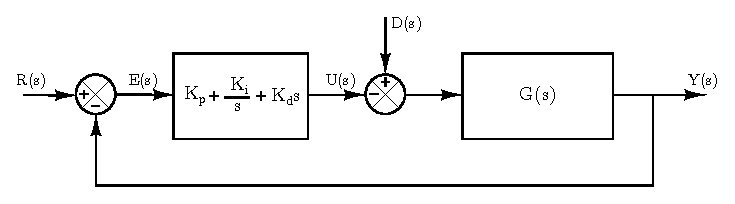
\includegraphics[width=8cm]{images/PIDcontroller.eps}
% \end{center}
% \begin{columns}
% \begin{column}{0.5\textwidth}
% Ventajas:
% \begin{itemize}
%   \item Elimina error de estado estacionario (I).
%   \item Elimina efecto de las perturbaciones (I).
%   \item Es anticipativo (D).
%   \item Tiene una acción inmediata (P).
% \end{itemize}
% \end{column}
% \begin{column}{0.5\textwidth}
% Desventajas:
% \begin{itemize}
%   \item Tiene un polo en el origen (genera inestabilidad).
%   \item La parte derivativa amplifica el ruido.
% \end{itemize}
% \end{column}
% \end{columns}
% \end{frame}

% \begin{frame}[<+->]\frametitle{Sintonización de Controladores}
% \textbf{Cómo encontrar los valores $K_p$, $K_i$, $K_d$?} No existe una manera única de encontrarlos! Existen muchos métodos:
% \begin{itemize}
%   \item Experimental.
%   \item Análisis de una F.T.
%   \item Técnicas de optimización.
%   \item Lugar geométrico de las raíces.
%   \item Compensación en frecuencia.
% \end{itemize}
% \end{frame}

% \begin{frame}[c]\frametitle{Ejemplo: Control PID de un Sistema de Segundo Orden}
% \footnotesize
% Considere el siguiente lazo de control:
% \begin{center}
%   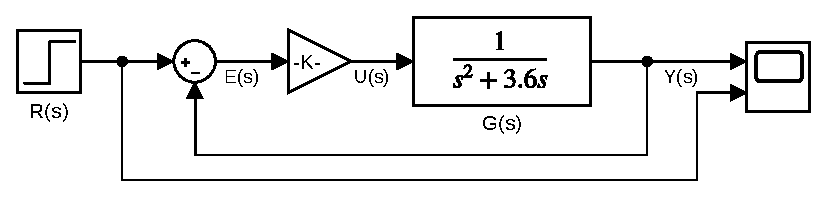
\includegraphics[width=8cm]{images/example2.eps}
% \end{center}
% \vspace*{-5mm}
% \begin{enumerate}
%   \item Calcule el valor de la ganancia $K_p$ para obtener un sobrepico de 10\% ante una entrada paso unitaria. Realice la simulación y verifique el resultado.
%   \item Considere ahora el sistema $G(s) = \frac{1}{s^2 + 3.6s + 1}$. Cómo cambia la respuesta al simular el sistema con la ganancia encontrada anteriormente?
%   \item Usando prueba y error, encuentre ganancias $K_p$ y $K_i$ de un control PI que mejore la respuesta del nuevo sistema.
%   \item Usando prueba y error, encuentre ganancias $K_p$ y $K_d$ de un control PD que mejore la respuesta del nuevo sistema.
%   \item Usando prueba y error, encuentre ganancias $K_p$, $K_i$ y $K_d$ de un control PID que mejore la respuesta del nuevo sistema.
% \end{enumerate}
% \end{frame}

\end{document}